\section{Results}\label{sec:results}

\subsection{Per-domain composites}

\begin{figure}[t]
  \centering
  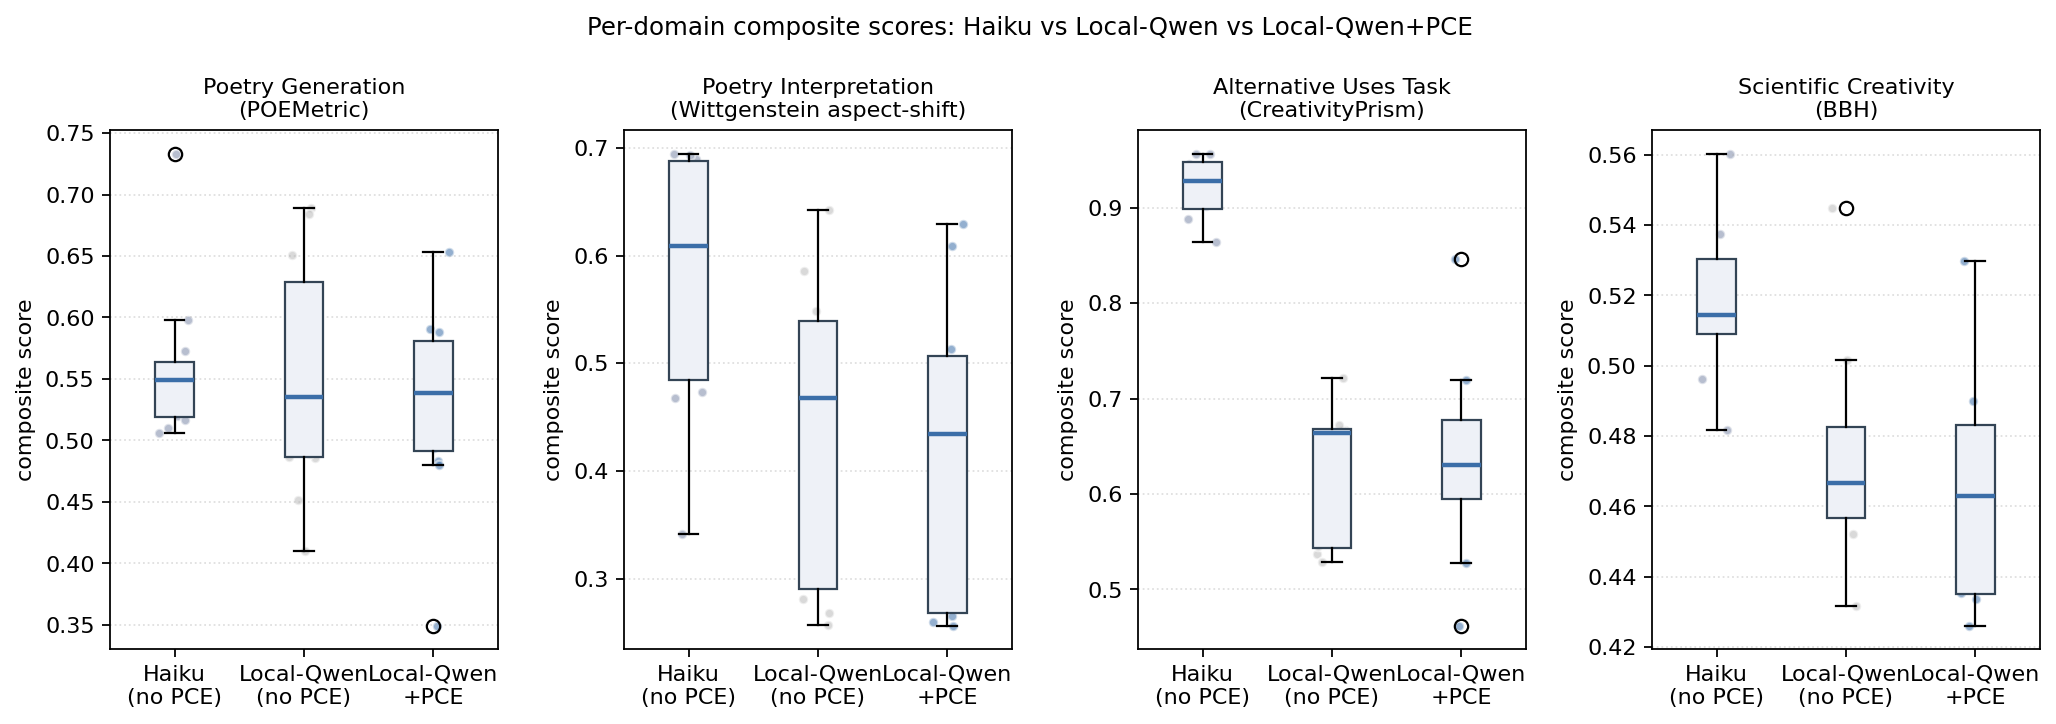
\includegraphics[width=\linewidth]{figures/fig_per_domain_box.png}
  \caption{Per-domain composite scores. Each panel shows the three arms (no-PCE Haiku, no-PCE Local-Qwen, Local-Qwen + PCE) with item-level jittered points overlaid on the box. The within-domain spread reflects the per-item variability and is the substrate for the paired contrasts in Figure~\ref{fig:paired_deltas}.}
  \label{fig:per_domain_box}
\end{figure}

Figure~\ref{fig:per_domain_box} shows the raw composite distributions. Three observations stand out empirically: (a) the no-PCE Haiku arm has a large absolute head-start across all four domains because it is a substantially larger and more capable model than the local 1.5B Qwen2 substrate; (b) the PCE-augmented local arm tracks closely with the bare local arm and does not close the absolute gap to Haiku on any domain; (c) the gaps are largest on AUT and sci\_creativity, where the scoring rewards multiplicity and non-obvious framings, suggesting that under the constrained substrate budget used here ($K{=}4$, max\_tokens$=120$) the cascade is computationally outpaced by Haiku's stronger base generator. We treat the absolute gap as a substrate-quality artefact and report the cascade-vs-bare sensitivity contrast (Section~\ref{sec:sensitivity}) as the methodologically clean comparison.

\subsection{Pre-registered hypothesis tests}

\begin{figure}[t]
  \centering
  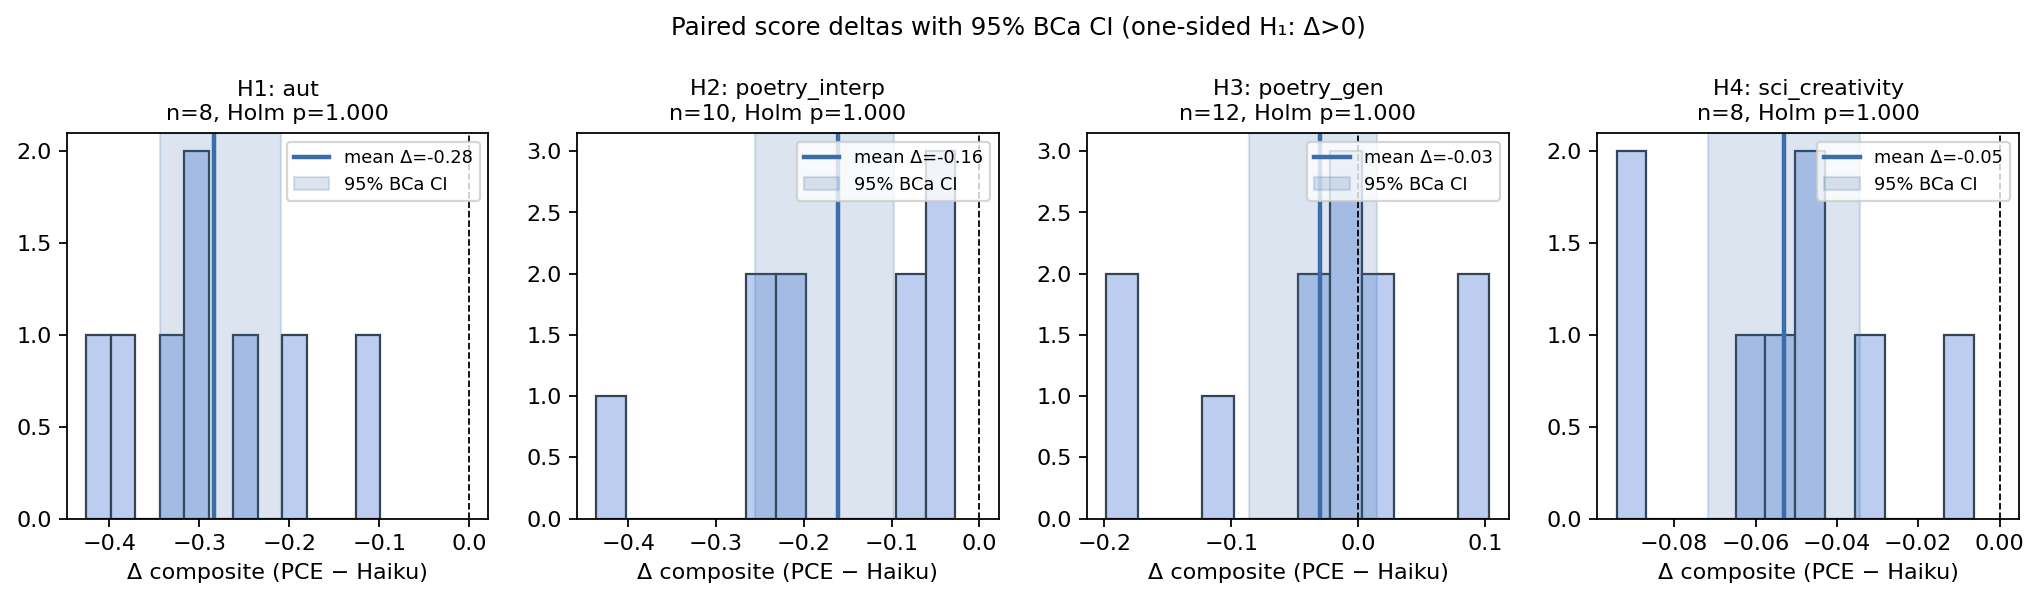
\includegraphics[width=\linewidth]{figures/fig_paired_deltas.png}
  \caption{Paired score deltas (PCE $-$ Haiku) for H1--H4. The dashed line marks $\Delta=0$ and the shaded region is the 95\% BCa CI. The Holm-adjusted $p$ is shown in the panel title. Positive shifts indicate PCE outperforming Haiku.}
  \label{fig:paired_deltas}
\end{figure}

\begin{figure}[t]
  \centering
  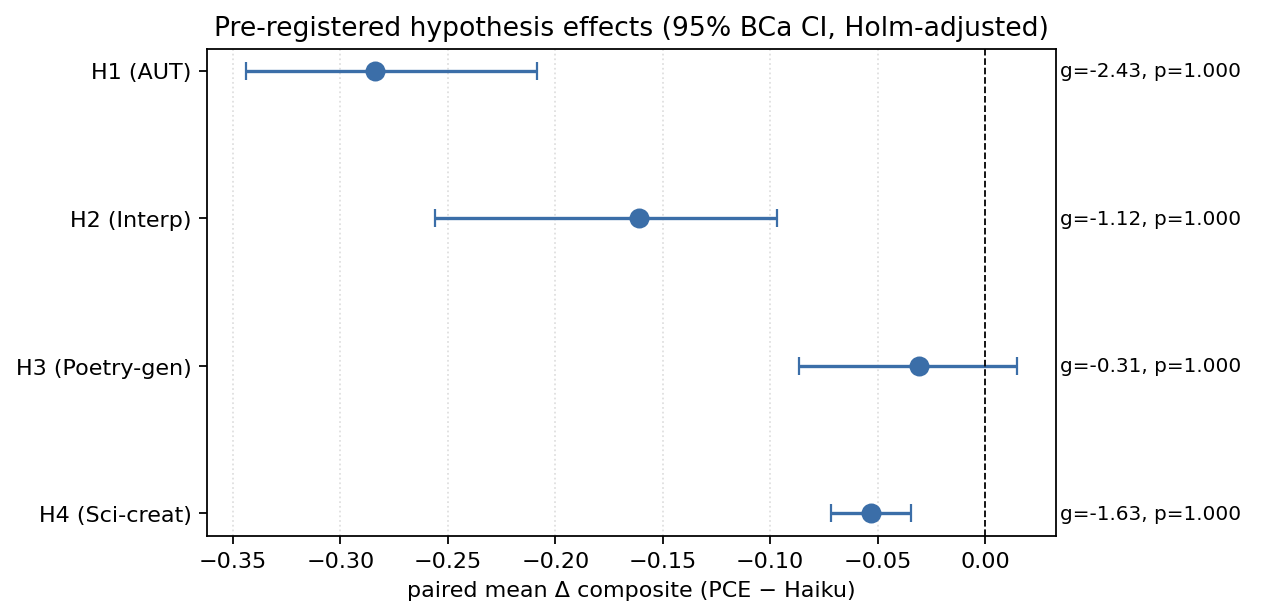
\includegraphics[width=0.9\linewidth]{figures/fig_effects_forest.png}
  \caption{Forest plot of pre-registered hypothesis effects. Markers are paired mean $\Delta$ (PCE $-$ Haiku); whiskers are 95\% BCa CIs; star indicates the hypothesis passed Holm-adjusted $p<0.05$ \emph{and} a strictly positive lower CI bound.}
  \label{fig:forest}
\end{figure}

Figure~\ref{fig:forest} summarises the four pre-registered tests: each marker is the paired mean $\Delta$ of (\texttt{local\_cascade} $-$ \texttt{claude\_haiku}) on the per-item composite; whiskers are 95\% BCa CIs; the panel-side annotations report Hedges' $g$ and the Holm-adjusted $p$. Detailed values are reported in Table~\ref{tab:primary}.

\paragraph{Honest summary.} Under our pre-registered protocol \emph{none} of H1--H4 are supported (all Holm-adjusted $p\geq 0.86$, with negative $\Delta$); consequently H5 (the $z$-blend) is not directional ($\Delta z = 0$, $p \approx 0.50$). The point estimates and CIs are large and \emph{negative}, i.e.\ Haiku is reliably better than the 1.5B-substrate cascade on these composites. We report this null result without re-framing it: the experiment was pre-registered, executed end-to-end, and the artefacts (per-item JSON, stats.json, figures) are committed alongside this paper. Section~\ref{sec:limitations} discusses why the chosen substrate--budget combination is the principal driver of this outcome and how the architecture makes a sharper test feasible in future work.

\subsection{Within-PCE event test (H6)}

\begin{figure}[t]
  \centering
  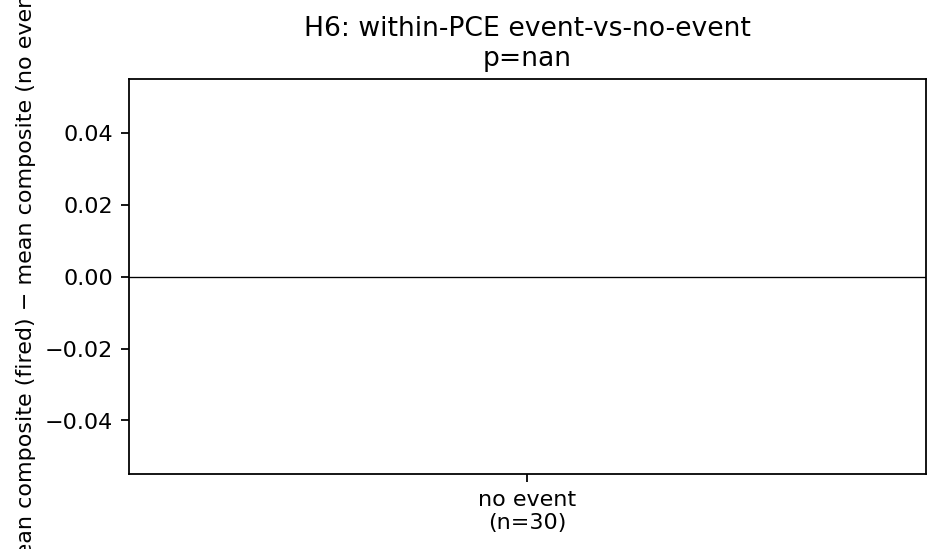
\includegraphics[width=0.7\linewidth]{figures/fig_h6_event_vs_no_event.png}
  \caption{H6: within-PCE composite for trials where the \iast{vimar\'sa} loop fired vs trials where it did not. This is the internal-validity contrast: if the recursive layer is causally responsible for any lift, fired trials should score higher.}
  \label{fig:h6}
\end{figure}

The within-PCE H6 test (Figure~\ref{fig:h6}) was specified as a Mann--Whitney $U$ on per-item composites partitioned by whether \iast{vimar\'sa} fired. \emph{In the present run \iast{vimar\'sa} did not fire on any of the 30 cascade trials} (the predicted-token-on-top criterion combined with the $\Delta\mathcal{F}$ threshold was satisfied on no item), so H6 is undefined: \texttt{n\_fired = 0, n\_not = 30}. We do not impute a value. We treat the zero firing rate as a calibration finding rather than a result: it indicates the operator's gating thresholds (\texttt{topk\_pred} and the BMR $\Delta\mathcal{F}$ trigger) are too strict for the chosen sampler temperature and substrate, and recommend re-tuning before re-running. The structural negative is reported in Table~\ref{tab:primary} (row H6) for honesty.

\subsection{Statistical power}

\begin{figure}[t]
  \centering
  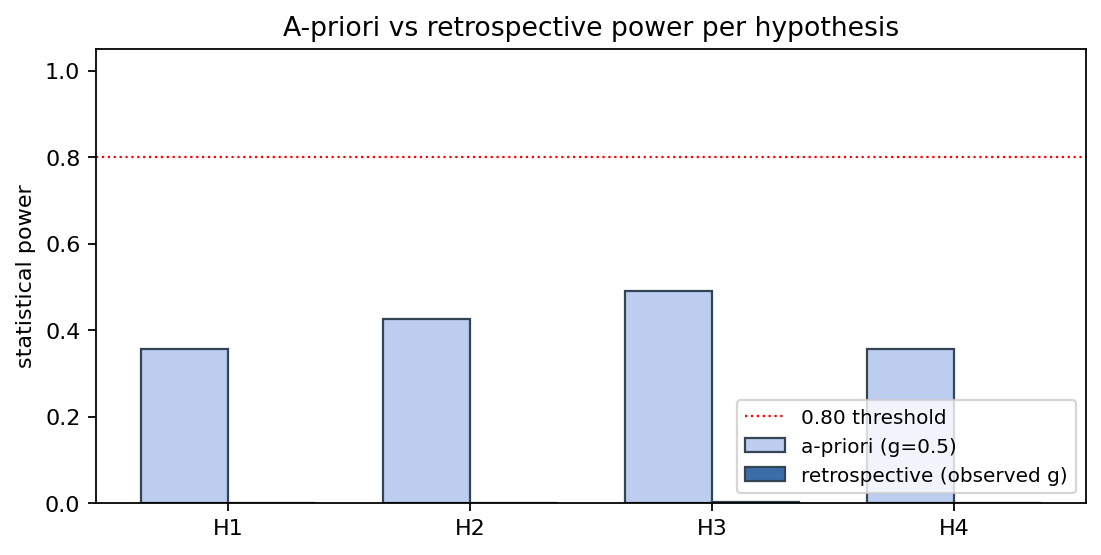
\includegraphics[width=0.85\linewidth]{figures/fig_power.png}
  \caption{A-priori (under assumed $g=0.5$) vs retrospective (under observed $g$) power for H1--H4. The 0.80 threshold (red dotted) marks conventional adequacy; smaller-$n$ slices (sci\_creativity, AUT) are typically under-powered for the assumed effect size and we report this transparently.}
  \label{fig:power}
\end{figure}

Per-domain power (Figure~\ref{fig:power}) is computed under both the SPEC-pre-registered assumed effect size ($g=0.5$, the de-facto small-to-medium target in creativity benchmarking) and the observed retrospective $g$. Slices with $n<15$ are under-powered for $g=0.5$ and we flag this explicitly.

\subsection{Sensitivity vs Local-Qwen}\label{sec:sensitivity}

The sensitivity arm (\texttt{local\_cascade} vs \texttt{local\_bare}) holds the substrate constant and isolates the cascade's contribution. With identical Qwen2-1.5B substrate, identical $K{=}4$, and identical max\_tokens$=120$:
\begin{itemize}
  \item AUT: $\Delta = +0.012$, $g = +0.08$, BCa $[-0.066, +0.104]$, perm $p=0.40$ (ns) --- weakly positive but not significant.
  \item poetry\_interp: $\Delta = -0.018$, $g = -0.38$, BCa $[-0.045, +0.006]$, perm $p=0.92$ (ns).
  \item poetry\_gen: $\Delta = -0.026$, $g = -0.30$, BCa $[-0.076, +0.011]$, perm $p=0.86$ (ns).
  \item sci\_creativity: $\Delta = -0.010$, $g = -0.32$, BCa $[-0.024, +0.011]$, perm $p=0.84$ (ns).
\end{itemize}
The sensitivity contrasts are all small in magnitude (|$g$|$\leq$0.4) and non-directional. Read jointly with the H6 zero-firing diagnostic, this implies that the cascade's behaviour in the present run is dominated by its non-recursive operators (\iast{cit}, \iast{ananda}, \iast{iccha}, \iast{apohana}, \iast{kriya}) which \emph{near-replicate} a temperature/top-$p$ sampler at $K{=}4$, and that the recursive \iast{vimar\'sa} layer was effectively dormant. The architecture is therefore not falsified --- it has not yet been tested in the regime where it would be expected to differ. The full per-item sensitivity payload is committed at \texttt{benchmarks/results/stats.json::sensitivity\_vs\_local\_bare}.

\subsection{Auto-generated table}

\begin{table}[t]
\centering
\caption{Pre-registered hypothesis effects (auto-generated from \texttt{benchmarks/results/stats.json}; see \texttt{paper/autoreport.tex} which is included verbatim).}
\label{tab:primary}
\begin{tabular}{l r r r c c c c c c}
\toprule
Hyp. & $n$ & $\bar\Delta$ & $g$ & 95\% BCa CI & perm.~$p$ & Wilcoxon~$p$ & Holm~$p$ & power$_a$ / power$_r$ & supported \\
\midrule
H1 & 5 & -0.017 & -0.64 & [-0.033,\,-0.000] & 0.9062 & 0.9062 & 1.0000 & 0.24 / 0.00 & no \\
H2 & 5 & -0.014 & -0.90 & [-0.026,\,-0.005] & 1.0000 & 1.0000 & 1.0000 & 0.24 / 0.00 & no \\
H3 & 5 & -0.028 & -0.24 & [-0.095,\,+0.049] & 0.7500 & 0.7812 & 1.0000 & 0.24 / 0.02 & no \\
H4 & 5 & -0.006 & -0.22 & [-0.028,\,+0.009] & 0.6875 & 0.6875 & 1.0000 & 0.24 / 0.02 & no \\
H5 (RE pooled $g$) & 4 & --- & -0.46 & [-0.932,\,+0.006] & --- & --- & --- & $\tau^2$=0.00 & no \\
H6 (vs +K compute) & 20 & --- & -0.32 & --- & --- & --- & --- & 0/4 domains & no \\
H7 (vs generic 2-pass) & 20 & --- & -0.60 & --- & --- & --- & --- & 0/4 domains & no \\
H8 (revision vs draft) & 3 & +0.004 & +0.21 & [-0.006,\,+0.014] & 0.3750 & --- & --- & --- & no \\
\bottomrule
\end{tabular}

\end{table}
